\section{Результаты и обсуждение}

\subsection{Подготовка и проведение масс-спектрометрических измерений}
Тут что-нибудь про бактерий напиать.
Были отсняты масс-спектры 30 культур. Из них 6 были не фракционированы, остальные были разделены на 6 фракций. Разделение на фракции позволило идентифицировать пептиды, которые не были бы идентифицированы при обычном поиске, из-за того, что на измерения MS/MS спектра были бы отобраны более высоко представленные пептиды. Количество отснятых спектров для каждой культуры представлены в таблице.

\subsection{Подготовка баз}
Скаченная с NCBI аннотация содержала 4103 аннотированных белок-кодирующих последовательностей. После добавления контаминант и decoy-последовательностей получилась белковая база, состоящая из 8258 последовательностей. После транслирования генома в 6 рамках и исключения коротких последовательностей получилось 74488 белок-кодирующих последовательностей. В результате добавления контаминант и decoy-последовательностей, получилась геномная база, состоящая из 149028 последовательностей. Исключение коротких последовательностей из геномной базы позволило ускорить поиск; снизить пороговые значения идентификации, тем самым повысив чувствительность подхода. Минимальная длинна аннотированного белка \ti{W-148} составляет 84 аминокислоты, таким образом, исключение рамок длинной меньше чем 33 аминокислоты не должно привести к потерям при идентификации.

\subsection{Идентификация белков и пептидов}
Поиск проходил при помощи поисковых маших Mascot и X!Tandem. Объединение результатов поиска и перерасчет FDR был произведен в Scaffold. Против белковой базы было идентифицировано 32054 пептида (1041059 psm), против геномной базы 36502 уникальных пептида (1131085 psm). Пересечение идентифицированных пептидов представлено на рисунке \ref{Identification}. Часть пептидов идентифицирована против белковой базы и не идентифицирована против более полной полной геномной базы. Это связано с различными пороговыми скорингами при поиске против баз разных размеров. 
После вычитания результатов поиска против белковой базы из результатов поиска против геномной базы получилось 6015 GSSP (Genome search specific peptides).  После исключения пептидов представленных в аннотированном геноме и идентифицированных только против геномной базы, осталось 1397 GSSP. Наличие таких пептидов, идентифицируемых только против геномной базы и представленных в аннотации, связано с пересчетом FDR: при отдельном рассмотрении результатов идентификации каждой поисковой машины таких эффектов не возникает.  После исключения GSSP, представленных только в одной культуре, осталось 425 пептидов. Результаты интерпретации GSSP при таких фильтрах: 16 новый ORF, и 304 гена с корректированным положением старта.  
Пептидов, интерпретируемых как пептиды перед аннотированным стартом примерно в 8 раз больше, чем пептидов, относящихся к новым генам. Такой разброс может быть связан с тем, что пептидам относящимся к корректировке рамки проще пройти порог FDR. В самом деле, при пептидном и белковом FDR в 1\% и, примерно, 1000000 psm при размере базы в 4000 аминокислотных последовательностей, 10000 пептидов будут ложно-положительно идентифицированы. Если брать критерий 2 и более пептидов для идентификации белка, то такого количества пептидов будет достаточно для идентификации 5000 белков, если не учитывать белковой FDR. С учетом белкового FDR количество ложно-положительно идентифицированных белков должно быть не боле 40. Для этого достаточно 80 пептидов. Таким образом, в экспериментах с большим количеством исходных данных, белковый FDR становится более жестким критерием, чем пептидный. Соответственно, GSSP относящимся к корректировке рамки проще пройти белковый FDR, так как в этой рамке так же присутствуют пептиды из аннотированной части последовательности. В случае нового гена в "прохождение"\ белкового FDR участвуют только GSSP пептиды.

\begin{figure}[pH]
    \begin{center}
        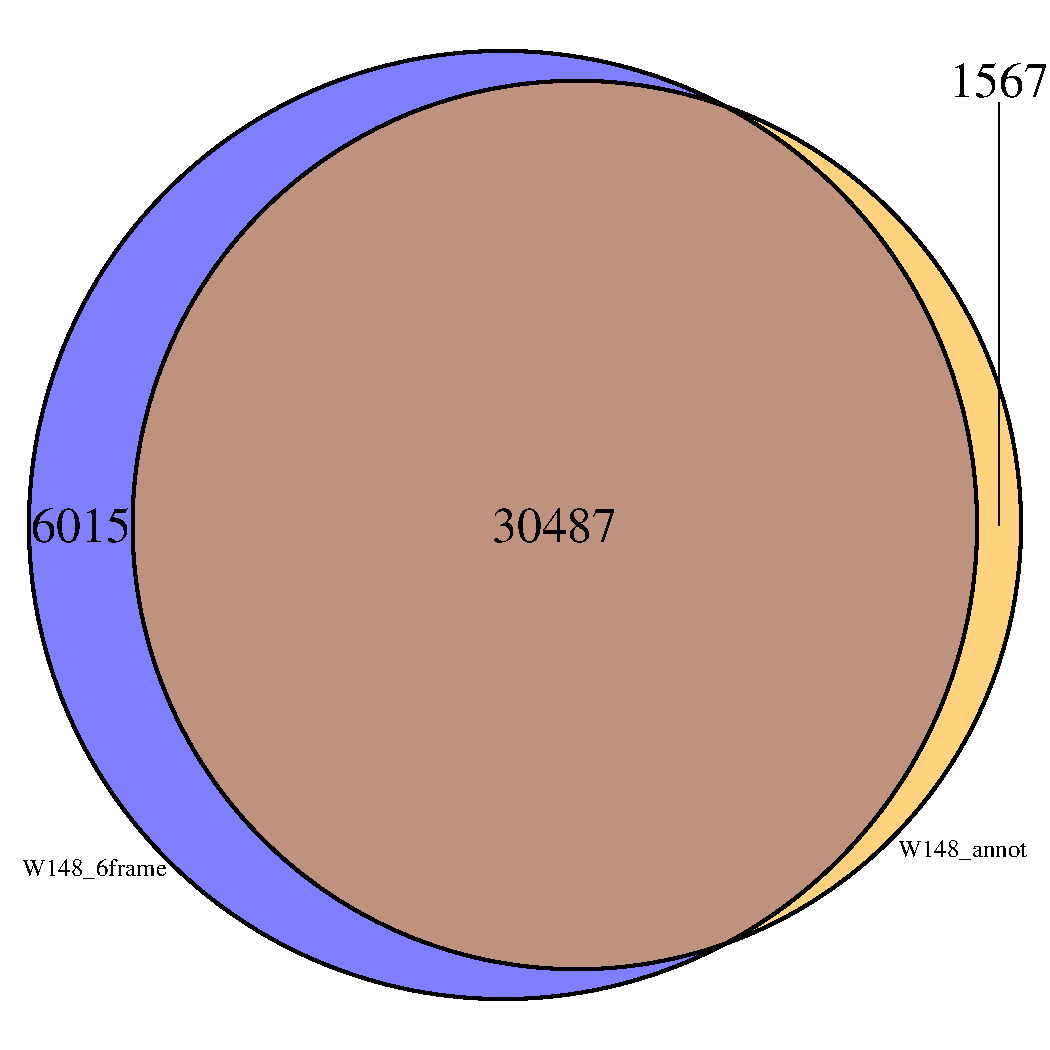
\includegraphics[width=0.9\linewidth]{Identification.pdf}
    \end{center}
\caption[foo bar]{Сравнение идентификаций против различных баз:
  \begin{enumerate*}%[label=\textit{\alph*)}]
    \item annot - количество уникальных пептидов идетифицированных против белковой базы
    \item 6frame - количество уникальных пептидов идетифицированных против геномной базы
  \end{enumerate*}.}
\label{Identification}
\end{figure}

Для подтверждения результатов были применены дополнительные критерии. После удаления PSM, ошибка идентификации которых составляет более трех стандартных отклонений в предположении о нормальном распределении ошибки идентификации всех PSM в интервале +/- 5 минут, остался 331 уникальный GSSP. Следует отметить, что на этом шаге отсекались пептиды, ошибка идентификации которых меньше, чем реальная точность приборов. Поэтому данный критерий отнесен к дополнительным. Затем была проведена фильтрация по времени выхода. После исключения 10\% наиболее отклоняющихся пептидов, остался 147 уникальный GSSP. 

Все GSSP были проверены на точное вхождение в базу NCBInr. Среди белков, в которых нашлись GSSP, не было найдено  таких, которые бы относились к организмам, которые ранее снимались на используемом масс-спектрометре. Таким образом можно исключить остаточную контаминацию на приборе и пробоподготовке. Так же были исключены 8 пептидов, которые присутствуют в аннотированных последовательность \ti{W-148} с учетом одной замены.

\subsection{Интерпретация новых событий}
\subsubsection{Новые ORF}
Было идентифицировано 16 новых ORF, в которых присутствует 2 и более уникальных GSSP. Из шестнадцати ORF пять пересекаются с аннотированными псевдогенами, одиннадцать лежат на комплиментарной цепи участков с аннотированными генами. У пяти из шестнадцати есть гомолог в \ti{H37Rv}. Гены всех \ti{M.tuberculosis} плотно расположены, и межгенные области либо отсутствуют, либо их длинна намного меньше длины гена, либо, если межгенник большой, в нем находится псевдолен. Поэтому не найдено новых генов, которые не относились бы к псевдогенам и лежали в межгенном пространстве.

Следует отметить, что причины по которым ген становится "псевдоегном"\ с точки зрения биологии и системы аннотации NCBI различны. Так, наиболее частыми причинами из-за которых участок генома аннотируется как псевдоген являются: фреймшифт (потеря или вставка не кратного трем числа нуклеотидов, в результате чего нарушается белковая последовательность), неполный ген (присутвствует только часть гена, в сравнении с гамологами), стоп-кодон по середине последовательности, низкое качество сборки (например, если ген находится на стыке контигов). Для всех идентифицированных псевдогенов была найдена "техническая"\ и "биологическая"\ причина, из-за которой они получили статус псевдогена. Пример идентифицированно псевдогена представлен на рисунке \ref{pseudo_1}.

\begin{figure}[ph!]
    \begin{center}
        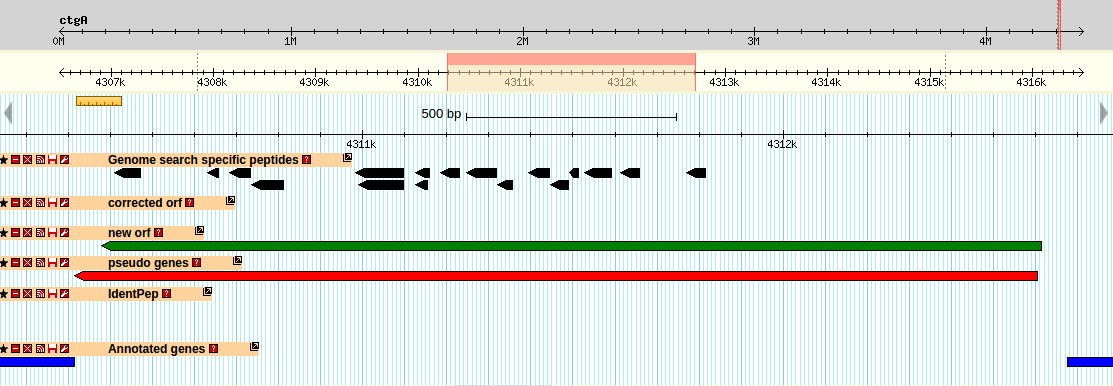
\includegraphics[width=1.2\linewidth, angle=-90]{pseudo_1.png}
    \end{center}
\caption[foo bar]{Идентифицированный псевдоген. Сними обозначены аннотированые гены, красным - псевдоген, зеленым - открытая рамка считывания, Genome search specific peptides - пептиды, идентифицируемы только про поиски против геномной базы}
\label{pseudo_1}
\end{figure}

\begin{figure}[ph!]
    \begin{center}
        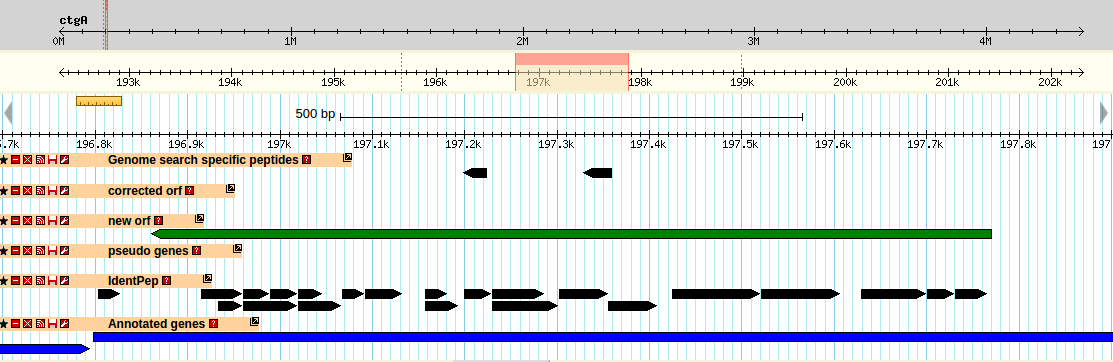
\includegraphics[width=1.2\linewidth, angle=-90]{comp_gene.png}
    \end{center}
\caption[foo bar]{ORF, лежащий на комплиментраной цепи к аннотированому и экспрессирующемуся гену. Сними обозначены аннотированые гены, IdentPep - идентифицрованные при поиске против белковой базы пептиды, красным - псевдоген, зеленым - открытая рамка считывания, Genome search specific peptides - пептиды, идентифицируемы только про поиски против геномной базы}
\label{comp_gene}
\end{figure}

\begin{figure}[ph!]
    \begin{center}
        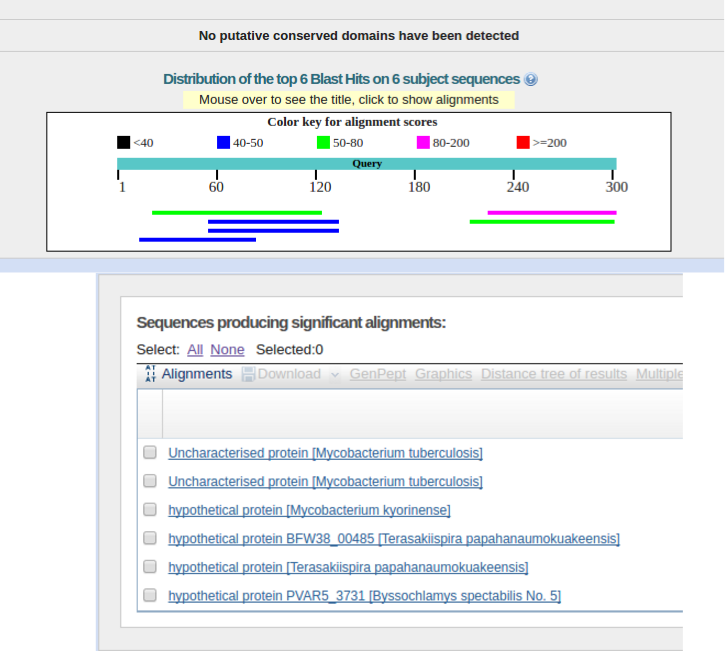
\includegraphics[width=1\linewidth]{comp_gene_blast.png}
    \end{center}
\caption[foo bar]{Результат поиска гомолога ORF, лежащей на комплиментарной цепи и предсталвенной на рисунке \ref{comp_gene}) против базы NCBInr с ипользованием алгоритма blast.}
\label{comp_gene_blast}
\end{figure}


В результате поиска против базы NCBInr при помощи алгоритма blust для десяти из одинналцати ORF, лежащих на комплиментарной цепи (пример такого ORF предствлен на рисунке \ref{comp_gene}) к аннотированным генам, были найдены гомологи. Эти гомологи были аннотированы как “гипотетический/предсказанный/непроверенный белок” другого штамма \ti{M.tuberculosis}. Косвенно результаты идентификации подтверждает тот факт, что все новые ORF лежат на комплиментарной цепи, а не в другом фрейме аннотированной. В самом деле, с пространственной точки зрения предположение, что транскрипт снимается с комплиментарной цепи выглядит более вероятным, чем предположение, что с одного транскрипта идет трансляция в двух фреймах двух разных аминокислотных последовательностей.

После применения дополнительных критериев фильтрации GSSP осталось шесть ORF с псевдогенами и один ORF на комплиментарной цепи.

\subsubsection{Корректировка положения аннотированного старта}
Всего 304 рамки содержат аннотированный ген и GSSP пептид. Из 304 308 содержат два и более GSSP. Эти рамки сравниили с гомологичными генами в \ti{H37Rv}. Из 38 36 совпадают с точностью до SAP, 2 рамки длинней у \ti{W-148}, чем у \ti{H37Rv}. Для этих 38 рамок были проверены пептиды, пересекающиеся аннотированный старт. Для 17 из 38 были найдены пептиды, содержащие в себе аннотированный старт (overlap-пептиды), для 7 были найдены стартовые пептиды из аннотации, для 3 были найдены как стартовые, так и аннотированные пептиды.

\subsubsection{Пептиды, содержащие аннотированный старт}
Для 17 из 38 рамок, содержащих аннотированный ген и два более GSSP, были найдены пептиды, содержащие в себе стартовую аминокислоту для аннотированного гена. Такой пептид представлен на рисунке \ref{overlap_pep}. Для 7 из 38 были найдены пептиды, являющиеся стартовыми для аннотированного гена. У 3 из 38 найдены как стартовые, так и overlap-пептиды, причем в этом месте не было сайта трипсинолиза.

\begin{figure}[h!]
    \begin{center}
        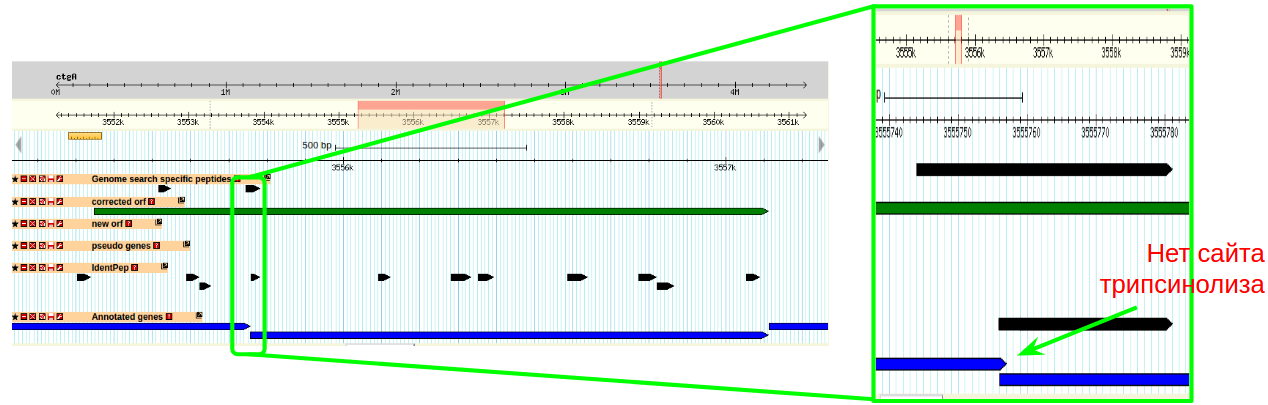
\includegraphics[width=1\linewidth]{overlap_pep.png}
    \end{center}
\caption[foo bar]{Ген с измененой рамкой считывания. Черным обозначены идентифицированные пептиды. Верхний глиф - GSSP, нижний - пептиды, идентифицированные при поиске против белковой базы. Идентифицирован как стартовый пептиы, так и overlap-пептид. Сайта трипсинолиза в этом месте нет. }
\label{overlap_pep}
\end{figure}



\newpage


































